%%%%%%%%%%%%%%%%%%%%%%%%%%%%%%%%%%%%%%%%%%%%%%%%%%%%%%%%%% 
\chapter{実行実験} \label{chap:experiment}
%%%%%%%%%%%%%%%%%%%%%%%%%%%%%%%%%%%%%%%%%%%%%%%%%%%%%%%%%% 
\section{実験概要}
論文\cite{adachi2023}では,SATソルバーを1回起動するだけで極小モデルを計算する手法が提案されたが,当該手法の実行性能に関する評価は十分に行われていなかった.同様に,本論文で提案する,SATソルバー1回起動による極大モデル計算方法についても,その性能は未評価である.そこで本節では,極小モデル計算の評価対象としてグラフ問題である極小支配集合問題(Minimal Dominating Set: MDS)を,極大モデル計算の評価対象としてグラフ問題である極大独立集合問題(Maximal Independent Set: MIS)を用いる.
具体的には,論文\cite{koshimura2009minimal}で提案された極大モデル計算手法(MIS-basic)および極小モデル計算手法(MDS-basic),論文\cite{adachi2023}で提案された極小モデル計算手法(MDS-trans),ならびに本論文で提案する極大モデル計算手法(MIS-trans)を比較対象とし,これらの手法に対して実行実験を行うことで性能評価を行う.\\

\section{実験環境}
本実験における実行環境は以下の通りである.
\begin{itemize}
 \item 実行環境:Mac mini,Apple M4,32GB
 \item SATソルバー:$CaDiCaL~3.0.0$ 
 \item 使用言語:$Rust$ 
 \item 制限時間:1問当たり30分
\end{itemize}

\section{ベンチマーク}
今回の実行実験で使用するベンチマークは3行n列($n=1,2,...,19$)のGrid graphの全19問である.
ここで,Grid graphとは,整数格子上の点を頂点とし,上下左右に隣接する点同士を辺で結んだグラフである.\\
支配集合とは,グラフ \(G=(V,E)\) において,頂点集合 \(D\subseteq V\) が,全ての頂点を自分自身または隣接頂点で覆うとき,\(D\) を支配集合と呼ぶ.すなわち,任意の頂点 \(v\in V\) について
\[
v\in D \ \ \text{または}\ \ \exists u\in D\ \text{s.t.}\ \{u,v\}\in E
\]
が成り立つ.\\
独立集合とは,グラフ \(G=(V,E)\) において,頂点集合 \(I\subseteq V\) が集合内の頂点同士が隣り合わない性質を満たすとき,\(I\) を独立集合と呼ぶ.これは,
\[
\forall u,v\in I\ (u\neq v)\Rightarrow \{u,v\}\notin E
\]
で表される.

\begin{example}\rm
 図\ref{fig:grid-mds}に3$\times$4のGrid graphにおける極小支配集合(MDS)の例を,図\ref{fig:grid-mis}に3$\times$4のGrid graphにおける極大独立集合(MIS)の例を示す.

 \begin{figure}[ht]
  \centering
    % tikz/gridgraph.tex
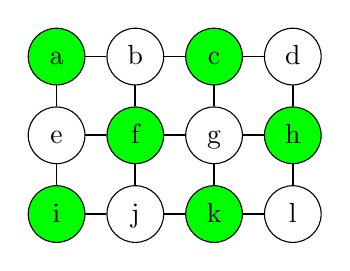
\begin{tikzpicture}[
  scale=1.0,
  v/.style={
    circle, draw,
    minimum size=7.2mm,
    inner sep=0pt,
    font=\normalsize,
    text height=1.6ex,
    text depth=.25ex
  },
  dom/.style={v, fill=red},                         % MDS vertex
  indep/.style={v, fill=green},      % MIS vertex
  both/.style={v, fill=gray!30, double, double distance=0.9pt}, % both
  edge/.style={draw, line width=0.65pt},
  domEdge/.style={draw, densely dashed, line width=0.9pt, dash pattern=on 2.2pt off 1.6pt}
]

% --- nodes (3x4) ---
\node[indep] (a) at (0,2) {a};
\node[v]   (b) at (1,2) {b};
\node[indep] (c) at (2,2) {c};
\node[v]     (d) at (3,2) {d};

\node[v]     (e) at (0,1) {e};
\node[indep] (f) at (1,1) {f};
\node[v]     (g) at (2,1) {g};
\node[indep]  (h) at (3,1) {h};

\node[indep]  (i) at (0,0) {i};
\node[v]     (j) at (1,0) {j};
\node[indep] (k) at (2,0) {k};
\node[v]     (l) at (3,0) {l};

% --- grid edges (solid) ---
\draw[edge] (a)--(b) (b)--(c) (c)--(d);
\draw[edge] (e)--(f) (f)--(g) (g)--(h);
\draw[edge] (i)--(j) (j)--(k) (k)--(l);

\draw[edge] (a)--(e) (e)--(i);
\draw[edge] (b)--(f) (f)--(j);
\draw[edge] (c)--(g) (g)--(k);
\draw[edge] (d)--(h) (h)--(l);

\end{tikzpicture}

  \caption{3$\times$4Grid graphのMIS}
  \label{fig:grid-mis}
 \end{figure}
\end{example}


 \begin{figure}[ht]
  \centering
    \input{tikz/gridgraph-mds}
  \caption{3$\times$4Grid graphのMDS}
  \label{fig:grid-mds}
 \end{figure}

\FloatBarrier

\section{CPU時間の比較}
表\ref{tab:mds-results}に MDSの既存手法と提案手法,表\ref{tab:mis-results}に MISの既存手法と提案手法の実行結果(各ベンチマークに対するCPU時間と得られた結果数)を示す.左に既存手法のCPU時間(秒)と得られた結果数,右に提案手法のCPU時間(秒)と得られた結果数を示す.各行において同一ベンチマークに対する両手法の計算時間結果を比較できる.また,赤文字で示されている結果は既存手法より短い時間で解けた問題である.MDS および MIS について,それぞれのカクタスプロットを図\ref{img:mds-plot},図\ref{img:mis-plot}に示す.横軸は Grid graph の列数 $n$,縦軸は各問題を解くのに要した CPU 時間である.同一の縦軸値に対して右側に位置するほど多くの問題を解けたことを意味し,下側に位置するほど短時間で解けたことを意味する.

図\ref{img:model-discovery}に SAT ソルバー起動に要したCPU時間とモデル計算に要したCPU時間の比較を示す.縦軸はCPU時間(秒),横軸は計算したモデルの数を示している.また,緑のプロットは既存手法でモデル計算に要した合計時間,赤のプロットは提案手法でモデル計算に要した合計時間,水色の棒グラフは既存手法においてSATソルバー起動でモデルを発見するために要した時間,青の棒グラフは既存手法においてSATソルバー起動でUNSATを出力するために要した時間である.

図\ref{img:model-times}に既存手法と提案手法のモデル計算に要したCPU時間推移の比較を示す.青のグラフが既存手法において各モデル計算に要した時間を,赤のグラフが提案手法において各モデル計算に要した時間を示している.このグラフでは上に行くほどモデル計算に時間を要したと言える.

まず表\ref{tab:mds-results}より,極小支配集合問題の全解列挙において既存手法は $3\times10$ まで解けたのに対し,提案手法は $3\times12$ まで解けた.さらに同一サイズの問題で比較すると,$3\times10$ において既存手法が 1361.24 秒を要したのに対し,提案手法は 3.620 秒で解けており,20 分以上の大幅な短縮が確認できる.

次に表\ref{tab:mis-results}より,極大独立集合問題の全解列挙において既存手法は $3\times13$ まで解けたのに対し,提案手法は $3\times18$ まで解けた.また $3\times13$ におけるCPU時間は,既存手法が 584.70 秒であるのに対し,提案手法は 0.36 秒であり,約 10 分の短縮が確認できる.

図\ref{img:mds-plot}および図\ref{img:mis-plot}においても,いずれの問題設定でも提案手法が既存手法よりも下側かつ右側に位置している.したがって,提案手法は既存手法に比べて,同一問題をより短時間で解けるだけでなく,制限時間内に解ける問題サイズの上限も拡大しており,総合的に高い性能を示すことが分かる.

また,図\ref{img:model-discovery}より,MDS および MIS のいずれにおいても,既存手法では頻繁な SAT ソルバーの起動がオーバーヘッドとなり,CPU時間全体の増加を招いていることが分かる.一方,提案手法ではソルバーの起動回数が大幅に抑制されているため,起動に伴うコストが低減され,効率的な計算が実現できている.

さらに,図\ref{img:model-times}より,提案手法は既存手法と比較して,各モデルを計算するのに要する時間がモデル数の増加に伴い短くなり,かつ安定して推移していることが読み取れる.これは,提案手法が大規模な解空間を持つ問題に対しても,高速に解を列挙し続けられることを示しており,CPU時間の短縮を裏付けるものである.

\begin{figure}[t]
  \centering

  %--- table ---
  \begin{minipage}{0.95\linewidth}
    \centering
    \captionof{table}{MDS のCPU時間と結果数}
    \label{tab:mds-results}
    \begin{tabular}{c|r|r|r|r}

\hline
& \multicolumn{4}{c}{極小モデル(極小支配集合)} \\
\hline
Benchmark & \multicolumn{2}{c|}{既存} & \multicolumn{2}{c}{提案} \\
\hline
& \multicolumn{1}{c|}{time} & \multicolumn{1}{c|}{results} & \multicolumn{1}{c|}{time} & \multicolumn{1}{c}{results}\\
\hline
\hline
grid3$\times$1  &    $<0.0$ &    2     &    \textcolor{red}{$<0.0$} &    2 \\
grid3$\times$2  &    $<0.0$ &    7     &    \textcolor{red}{$<0.0$} &    7 \\
grid3$\times$3  &    $<0.0$ &    16    &    \textcolor{red}{$<0.0$} &    16 \\
grid3$\times$4  &    $<0.0$ &    53    &    \textcolor{red}{$<0.0$} &    53 \\
grid3$\times$5  &    0.01 &    154   &    \textcolor{red}{$<0.0$} &    154 \\
grid3$\times$6  &    0.15 &    436   &    \textcolor{red}{0.01} &    436 \\
grid3$\times$7  &    1.86 &    1268  &    \textcolor{red}{0.03} &    1268 \\
grid3$\times$8  &    26.32 &    3660 &    \textcolor{red}{0.13} &    3660 \\
grid3$\times$9  &    182.35 &    10610 &    \textcolor{red}{0.58} &    10610 \\
grid3$\times$10 &    1361.24 &    30744 &    \textcolor{red}{3.620} &    30744 \\
grid3$\times$11 &     T.O. &    -   &    \textcolor{red}{24.84} &    89079 \\
grid3$\times$12 &     T.O. &    -   &    \textcolor{red}{207.90} &    258251 \\
grid3$\times$13 &     T.O. &    -   &     T.O. &    - \\
\hline
\end{tabular}


  \end{minipage}

  \vspace{6pt}

  %--- figure ---
  \begin{minipage}{0.95\linewidth}
    \centering
    \includegraphics[width=0.75\linewidth]{images/mds-plot.png}
    \captionof{figure}{MDS のCPU時間と結果数のプロット}
    \label{img:mds-plot}
  \end{minipage}
\end{figure}

\begin{figure}[t]
  \centering

  %--- table ---
  \begin{minipage}{0.95\linewidth}
    \centering
    \captionof{table}{MIS のCPU時間と結果数}
    \label{tab:mis-results}
    \begin{tabular}{c|r|r|r|r}

\hline
& \multicolumn{4}{c}{極大モデル(極大独立集合)} \\
\hline
Benchmark & \multicolumn{2}{c|}{既存} & \multicolumn{2}{c}{提案} \\
\hline
& \multicolumn{1}{c|}{time} & \multicolumn{1}{c|}{results} & \multicolumn{1}{c|}{time} & \multicolumn{1}{c}{results}\\
\hline
\hline
grid3$\times$1  &  $<0.0$ &  2     &  \textcolor{red}{$<0.0$} &  2 \\
grid3$\times$2  &  $<0.0$ &  4     &  \textcolor{red}{$<0.0$} &  4 \\
grid3$\times$3  &  $<0.0$ &  10    &  \textcolor{red}{$<0.0$} &  10 \\
grid3$\times$4  &  $<0.0$ &  18    &  \textcolor{red}{$<0.0$} &  18 \\
grid3$\times$5  &  $<0.0$ &  38    &  \textcolor{red}{$<0.0$} &  38 \\
grid3$\times$6  &  $<0.0$ &  74    &  \textcolor{red}{$<0.0$} &  74 \\
grid3$\times$7  &  0.01 &  148   &  \textcolor{red}{$<0.0$} &  148 \\
grid3$\times$8  &  0.01 &  290   &  \textcolor{red}{$<0.0$} &  290 \\
grid3$\times$9  &  0.04 &  578   &  \textcolor{red}{0.01} &  578 \\
grid3$\times$10 &  0.14 &  1156  &  \textcolor{red}{0.01} &  1156 \\
grid3$\times$11 &  0.36 &  2706  &  \textcolor{red}{0.05} &  2706 \\
grid3$\times$12 &  114.72 &  5518 &  \textcolor{red}{0.14} &  5518 \\
grid3$\times$13 &  584.70 &  11228 &  \textcolor{red}{0.36} &  11228 \\
grid3$\times$14 &  T.O. &  -   &  \textcolor{red}{1.52} &  22884 \\
grid3$\times$15 &  T.O. &  -   &  \textcolor{red}{5.26}&  46634 \\
grid3$\times$16 &  T.O. &  -   &  \textcolor{red}{23.53} &  94978 \\
grid3$\times$17 &  T.O. &  -   &  \textcolor{red}{110.72} &  193518 \\
grid3$\times$18 &  T.O. &  -   &  \textcolor{red}{756.59} &  394286 \\
grid3$\times$19 &  T.O. &  -   &  T.O. &  - \\
\hline
\end{tabular}


  \end{minipage}

  \vspace{6pt}

  %--- figure ---
  \begin{minipage}{0.95\linewidth}
    \centering
    \includegraphics[width=0.75\linewidth]{images/mis-plot.png}
    \captionof{figure}{MIS のCPU時間と結果数のプロット}
    \label{img:mis-plot}
  \end{minipage}
\end{figure}

\begin{figure}[t]
 \centering
 \begin{minipage}{0.95\linewidth}
  \centering
  \includegraphics[width=1.0\linewidth]{images/model_discovery.png}
  \caption{SATソルバー起動により要したCPU時間の比較}
  \label{img:model-discovery}
 \end{minipage}
 
 \vspace{10pt}

 \begin{minipage}{0.95\linewidth}
  \centering
  \includegraphics[width=1.0\linewidth]{images/model_times.png}
  \caption{既存手法と提案手法の計算したモデル数とCPU時間推移}
  \label{img:model-times}
  \end{minipage}
\end{figure}

\FloatBarrier

\section{CNFの変数,節の数とSATソルバー起動回数の比較}
表\ref{tab:mds-mis-cnf} に,Grid graph を CNF として定式化した際の変数数と節数を示す.varsが変数の数,clausesが節の数を示している.また,提案手法ではCNFを変換した後の変数,節の数が示されている.各行において同一ベンチマークに対する両手法の変数,節の数を比較できる.

表\ref{tab:c-solver}に,各計算手法における SAT ソルバー(CaDiCaL)の起動回数と,既存手法に対する提案手法の割合(\%)を示す.各行において同一ベンチマークに対する両手法のSATソルバー起動回数を比較できる.

表\ref{tab:mds-mis-cnf}より,MDSでの提案手法では,CNF の変換過程で Tseitin 変換を用いているため,補助変数が導入され,既存手法に比べて変数数が増加している.MIS の方が既存手法と提案手法の性能差が大きく現れている要因として,MDSでの提案手法では Tseitin 変換により CNF の構造が複雑化することでCPU時間が増加しやすい点が挙げられる.その結果として,MDS では変換によるCPU時間の高速化が MIS ほど顕著に表れにくいと考えられる.

表\ref{tab:c-solver}より,提案手法では,SAT ソルバーの起動回数が期待通り,得られた解の数と一致しており,解の列挙に対して無駄な起動が発生していないことが確認できる.具体例として $3\times8$ の Grid graph に着目すると,MDSの既存手法は計算過程で CaDiCaL を 17406 回起動しているのに対し,提案手法は 3660 回であり,提案手法は既存手法に比べて約21\%の起動回数で済んでいる.このように SAT ソルバー起動回数が減少していることは,ソルバー起動に伴うオーバーヘッドの削減につながるため,CPU時間の短縮に寄与していると考えられる.

\begin{table}[t]
 \centering
 \caption{MDS と MIS のCNFの変数数と節数の比較}
 \label{tab:mds-mis-cnf}
 \begin{tabular}{c|r|r|r|r|r|r|r|r}
\hline
& \multicolumn{4}{c|}{MDS(極小モデル)} & \multicolumn{4}{c}{MIS(極大モデル)} \\
\hline
& \multicolumn{2}{c|}{既存} & \multicolumn{2}{c|}{提案} & \multicolumn{2}{c|}{既存} & \multicolumn{2}{c}{提案} \\
\hline
Benchmark & vars & clauses & vars & clauses & vars & clauses & vars & clauses \\
\hline\hline
grid3$\times$1  & 3  & 3  & 10  & 16  & 3  & 2  & 3  & 5  \\
grid3$\times$2  & 6  & 6  & 26  & 60  & 6  & 7  & 6  & 13 \\
grid3$\times$3  & 9  & 9  & 42  & 110 & 9  & 12 & 9  & 21 \\
grid3$\times$4  & 12 & 12 & 58  & 160 & 12 & 17 & 12 & 29 \\
grid3$\times$5  & 15 & 15 & 74  & 210 & 15 & 22 & 15 & 37 \\
grid3$\times$6  & 18 & 18 & 90  & 260 & 18 & 27 & 18 & 45 \\
grid3$\times$7  & 21 & 21 & 106 & 310 & 21 & 32 & 21 & 53 \\
grid3$\times$8  & 24 & 24 & 122 & 360 & 24 & 37 & 24 & 61 \\
grid3$\times$9  & 27 & 27 & 138 & 410 & 27 & 42 & 27 & 69 \\
grid3$\times$10 & 30 & 30 & 154 & 460 & 30 & 47 & 30 & 77 \\
grid3$\times$11 & -  & -  & 170 & 510 & 33 & 52 & 33 & 85 \\
grid3$\times$12 & -  & -  & 186 & 560 & 36 & 57 & 36 & 93 \\
grid3$\times$13 & -  & -  & -   & -   & 39 & 62 & 39 & 101 \\
grid3$\times$14 & -  & -  & -   & -   & -  & -  & 42 & 109 \\
grid3$\times$15 & -  & -  & -   & -   & -  & -  & 45 & 117 \\
grid3$\times$16 & -  & -  & -   & -   & -  & -  & 48 & 125 \\
grid3$\times$17 & -  & -  & -   & -   & -  & -  & 51 & 133 \\
grid3$\times$18 & -  & -  & -   & -   & -  & -  & 54 & 141 \\
grid3$\times$19 & -  & -  & -   & -   & -  & -  & - & - \\
\hline
\end{tabular}

\end{table}

\begin{table}[t]
 \centering
 \caption{MDSとMISのSATソルバー起動回数の比較}
 \label{tab:c-solver}
 %========================
% MDS + MIS (merged)
%========================

\begin{tabular}{c|>{\raggedleft\arraybackslash}p{10mm} >{\raggedleft\arraybackslash}p{10mm}|r|>{\raggedleft\arraybackslash}p{10mm} >{\raggedleft\arraybackslash}p{10mm}|r}
\hline
& \multicolumn{3}{c|}{極小モデル(極小支配集合)} & \multicolumn{3}{c}{極大モデル(極大独立集合)} \\
\hline
\multicolumn{1}{c|}{Benchmark} &
\multicolumn{1}{c}{既存} &
\multicolumn{1}{c}{提案} &
\multicolumn{1}{c|}{割合[\%]} &
\multicolumn{1}{c}{既存} &
\multicolumn{1}{c}{提案} &
\multicolumn{1}{c}{割合[\%]} \\
\hline
 grid3$\times$1  & 7      & 2      & \textbf{28.6} & 6     & 2     & \textbf{33.3} \\
 grid3$\times$2  & 23     & 7      & \textbf{30.4} & 11    & 4     & \textbf{36.4} \\
 grid3$\times$3  & 62     & 16     & \textbf{25.8} & 23    & 10    & \textbf{43.5} \\
 grid3$\times$4  & 207    & 53     & \textbf{25.6} & 48    & 18    & \textbf{37.5} \\
 grid3$\times$5  & 594    & 154    & \textbf{25.9} & 101   & 38    & \textbf{37.6} \\
 grid3$\times$6  & 1743   & 436    & \textbf{25.0} & 203   & 78    & \textbf{38.5} \\
 grid3$\times$7  & 5502   & 1268   & \textbf{23.0} & 440   & 156   & \textbf{35.5} \\
 grid3$\times$8  & 17406  & 3660   & \textbf{21.0} & 907   & 321   & \textbf{35.3} \\
 grid3$\times$9  & 49864  & 10610  & \textbf{21.3} & 1848  & 651   & \textbf{35.2} \\
 grid3$\times$10 & 138754 & 30744  & \textbf{22.2} & 3808  & 1335  & \textbf{35.1} \\
 grid3$\times$11 & -      & 89079  & -    & 7896  & 2706  & \textbf{34.2} \\
 grid3$\times$12 & -      & 258251 & -    & 16127 & 5518  & \textbf{34.2} \\
 grid3$\times$13 & -      & -      & -    & 33281 & 11228 & \textbf{33.8} \\
 grid3$\times$14 & -      & -      & -    & -     & 22884 & -    \\
 grid3$\times$15 & -      & -      & -    & -     & 46634 & -    \\
 grid3$\times$16 & -      & -      & -    & -     & 94978 & -    \\
 grid3$\times$17 & -      & -      & -    & -     & 193518& -    \\
 grid3$\times$18 & -      & -      & -    & -     & 394286& -    \\
 grid3$\times$19 & -      & -      & -    & -     & -     & -    \\
\hline
\end{tabular}
\end{table}

% \begin{table}[htbp]
%  \centering
%  \caption{MDS のCPU時間と結果数}
%  \label{tab:mds-results}
%  \begin{tabular}{c|r|r|r|r}

\hline
& \multicolumn{4}{c}{極小モデル(極小支配集合)} \\
\hline
Benchmark & \multicolumn{2}{c|}{既存} & \multicolumn{2}{c}{提案} \\
\hline
& \multicolumn{1}{c|}{time} & \multicolumn{1}{c|}{results} & \multicolumn{1}{c|}{time} & \multicolumn{1}{c}{results}\\
\hline
\hline
grid3$\times$1  &    $<0.0$ &    2     &    \textcolor{red}{$<0.0$} &    2 \\
grid3$\times$2  &    $<0.0$ &    7     &    \textcolor{red}{$<0.0$} &    7 \\
grid3$\times$3  &    $<0.0$ &    16    &    \textcolor{red}{$<0.0$} &    16 \\
grid3$\times$4  &    $<0.0$ &    53    &    \textcolor{red}{$<0.0$} &    53 \\
grid3$\times$5  &    0.01 &    154   &    \textcolor{red}{$<0.0$} &    154 \\
grid3$\times$6  &    0.15 &    436   &    \textcolor{red}{0.01} &    436 \\
grid3$\times$7  &    1.86 &    1268  &    \textcolor{red}{0.03} &    1268 \\
grid3$\times$8  &    26.32 &    3660 &    \textcolor{red}{0.13} &    3660 \\
grid3$\times$9  &    182.35 &    10610 &    \textcolor{red}{0.58} &    10610 \\
grid3$\times$10 &    1361.24 &    30744 &    \textcolor{red}{3.620} &    30744 \\
grid3$\times$11 &     T.O. &    -   &    \textcolor{red}{24.84} &    89079 \\
grid3$\times$12 &     T.O. &    -   &    \textcolor{red}{207.90} &    258251 \\
grid3$\times$13 &     T.O. &    -   &     T.O. &    - \\
\hline
\end{tabular}


% \end{table}

% \begin{figure}[h]
%  \centering
%  \includegraphics[scale=0.6]{images/mds-plot.png}
%  \caption{MDS のプロット}
%  \label{img:mds-plot}
% \end{figure}



% \begin{table}[h]
%  \centering
%  \caption{MIS のCPU時間と結果数}
%  \label{tab:mis-results}
%  \begin{tabular}{c|r|r|r|r}

\hline
& \multicolumn{4}{c}{極大モデル(極大独立集合)} \\
\hline
Benchmark & \multicolumn{2}{c|}{既存} & \multicolumn{2}{c}{提案} \\
\hline
& \multicolumn{1}{c|}{time} & \multicolumn{1}{c|}{results} & \multicolumn{1}{c|}{time} & \multicolumn{1}{c}{results}\\
\hline
\hline
grid3$\times$1  &  $<0.0$ &  2     &  \textcolor{red}{$<0.0$} &  2 \\
grid3$\times$2  &  $<0.0$ &  4     &  \textcolor{red}{$<0.0$} &  4 \\
grid3$\times$3  &  $<0.0$ &  10    &  \textcolor{red}{$<0.0$} &  10 \\
grid3$\times$4  &  $<0.0$ &  18    &  \textcolor{red}{$<0.0$} &  18 \\
grid3$\times$5  &  $<0.0$ &  38    &  \textcolor{red}{$<0.0$} &  38 \\
grid3$\times$6  &  $<0.0$ &  74    &  \textcolor{red}{$<0.0$} &  74 \\
grid3$\times$7  &  0.01 &  148   &  \textcolor{red}{$<0.0$} &  148 \\
grid3$\times$8  &  0.01 &  290   &  \textcolor{red}{$<0.0$} &  290 \\
grid3$\times$9  &  0.04 &  578   &  \textcolor{red}{0.01} &  578 \\
grid3$\times$10 &  0.14 &  1156  &  \textcolor{red}{0.01} &  1156 \\
grid3$\times$11 &  0.36 &  2706  &  \textcolor{red}{0.05} &  2706 \\
grid3$\times$12 &  114.72 &  5518 &  \textcolor{red}{0.14} &  5518 \\
grid3$\times$13 &  584.70 &  11228 &  \textcolor{red}{0.36} &  11228 \\
grid3$\times$14 &  T.O. &  -   &  \textcolor{red}{1.52} &  22884 \\
grid3$\times$15 &  T.O. &  -   &  \textcolor{red}{5.26}&  46634 \\
grid3$\times$16 &  T.O. &  -   &  \textcolor{red}{23.53} &  94978 \\
grid3$\times$17 &  T.O. &  -   &  \textcolor{red}{110.72} &  193518 \\
grid3$\times$18 &  T.O. &  -   &  \textcolor{red}{756.59} &  394286 \\
grid3$\times$19 &  T.O. &  -   &  T.O. &  - \\
\hline
\end{tabular}


% \end{table}

% \begin{figure}[h]
%  \centering
%  \includegraphics[scale=0.6]{images/mis-plot.png}
%  \caption{MIS のプロット}
%  \label{img:mis-plot}
% \end{figure}


